\section{Regeln und Regelmengen}
Auf die Planknoten müssen während der Enumeration Regeln angewendet werden. Diese Regeln sind im vorliegenden Prototypen als \texttt{Rules} und \texttt{Regelmengen} abgelegt.

\subsection{Regelmengen}
Mehrere Regeln werden in einer Regelmenge zusammengefasst.
Insgesamt wurden vier unterschiedliche Regelmenegen implementiert: \textit{RS-B0}, \textit{RS-B1}, \textit{RS-B2} und \textit{GraphRule}.
Alle Mengen basieren auf den von Pellenkoft et al. vorgestellten Regelmengen und dem von \cite{shanbhag2014optimizing} implementierten GraphRule.

\begin{figure}[ht]
  \centering
  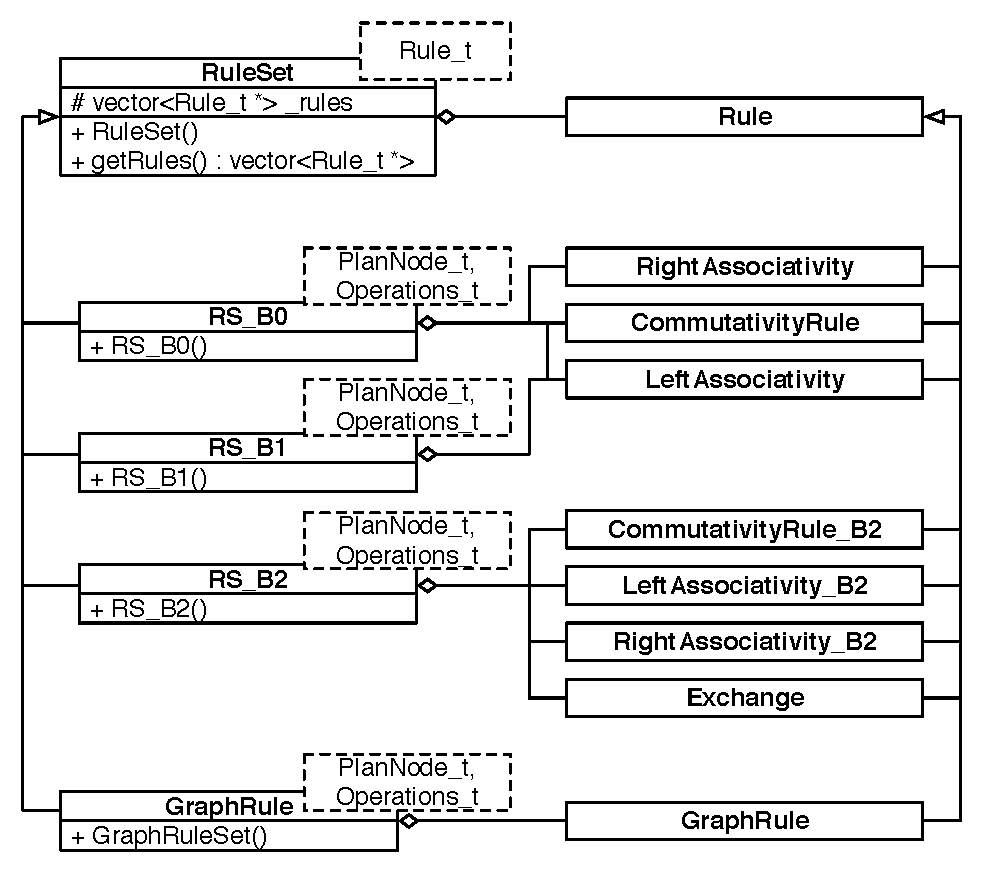
\includegraphics[scale=0.75]{04_Implementierung/00_media/RuleSets.pdf}
  \caption{Klassendiagramm: Regelmengen und Regeln}
  \label{RuleSetClass}
\end{figure}

\subsubsection{Implementierung}
\label{sec:RuleImplementation}

Alle Regelmengen erben von der Klasse \texttt{RuleSet}, die die Methode \texttt{getRules()} implementiert, mit deren Hilfe ein Vektor von Regeln ausgegeben wird. Je nach Regelmenge können andere Regeln vorhanden sein. Eine Übersicht über Regeln und deren Zuordnung zu Regelsets findet sich in Abb. \ref{RuleSetClass}.

Die einzelnen Regeln bei der Erstellung einer Regelmenge instantiiert, sind dem Vector \texttt{\_rules} zugeordnet. Die Sammlung der Regeln in einem Vector ist möglich, da alle Regeln von der abstrakten Klasse \texttt{Rule} erben. 

Konkret ist dem Regelset \textit{RS-B0} die Regel \texttt{RightAssociativity}, \texttt{Commutativity} und \texttt{LeftAssociativity} zugeordnet, dem Regelset \textit{RS-B1} \textit{Left Associativity} und \textit{Commutativity}. Dem Regelset \textit{RS-B2} sind die Varianten von Kommutativität, linker und rechter Assozativität, die speziell für diese Regelmenge erstellt wurden, zugeordnet, ebenso wie die \texttt{Exchange} Regel. Der \textit{Graph Rule} wird nur für \textit{RS-Graph} benötigt.

\subsubsection{Erweiterbarkeit}
Die Erweiterung der Regelmengen ist in verschiedenen Dimensionen möglich. Neue Funktionen können für die Regelmengen implementiert werden, ebenso ist die Erstellung neuer Regelmengen möglich.

Auf funktionaler Ebene ist es vorstellbar, dass die Reihenfolge der Regeln dynamisiert werden. Aktuell ist es nur möglich, die Regeln in Form eines Vektors auszugeben, dessen Reihenfolge immer gleich ist. Da alle konkreten Regelmengen von der selben Klasse \texttt{RuleSet} erben, ist die Implementierung einer anpassbaren Reihenfolge leicht möglich und muss für alle Klassen nur einmal vorgenommen werden.


Auch das Hinzufügen von neuen Regeln zu bestehenden Regelmengen oder die Erweiterung von bestehenden Regelmengen ist möglich. Beispielsweise kann von bestehenden Regelmengen geerbt wird bzw. neue Regeln und deren Regelmengen durch die Implementierung der standardisierten Interfaces \textit{RuleSet} entstehen.

Die Erweiterbarkeit konnte mit der Implementierung der Regelmenge  \textit{Graph Rule} unter Beweis gestellt werden, da diese Regelmenge erst später entwickelt wurde und auf die bestehende Infrastruktur aufsetzte.




\subsection{Regeln}

\begin{figure}[ht]
  \centering
  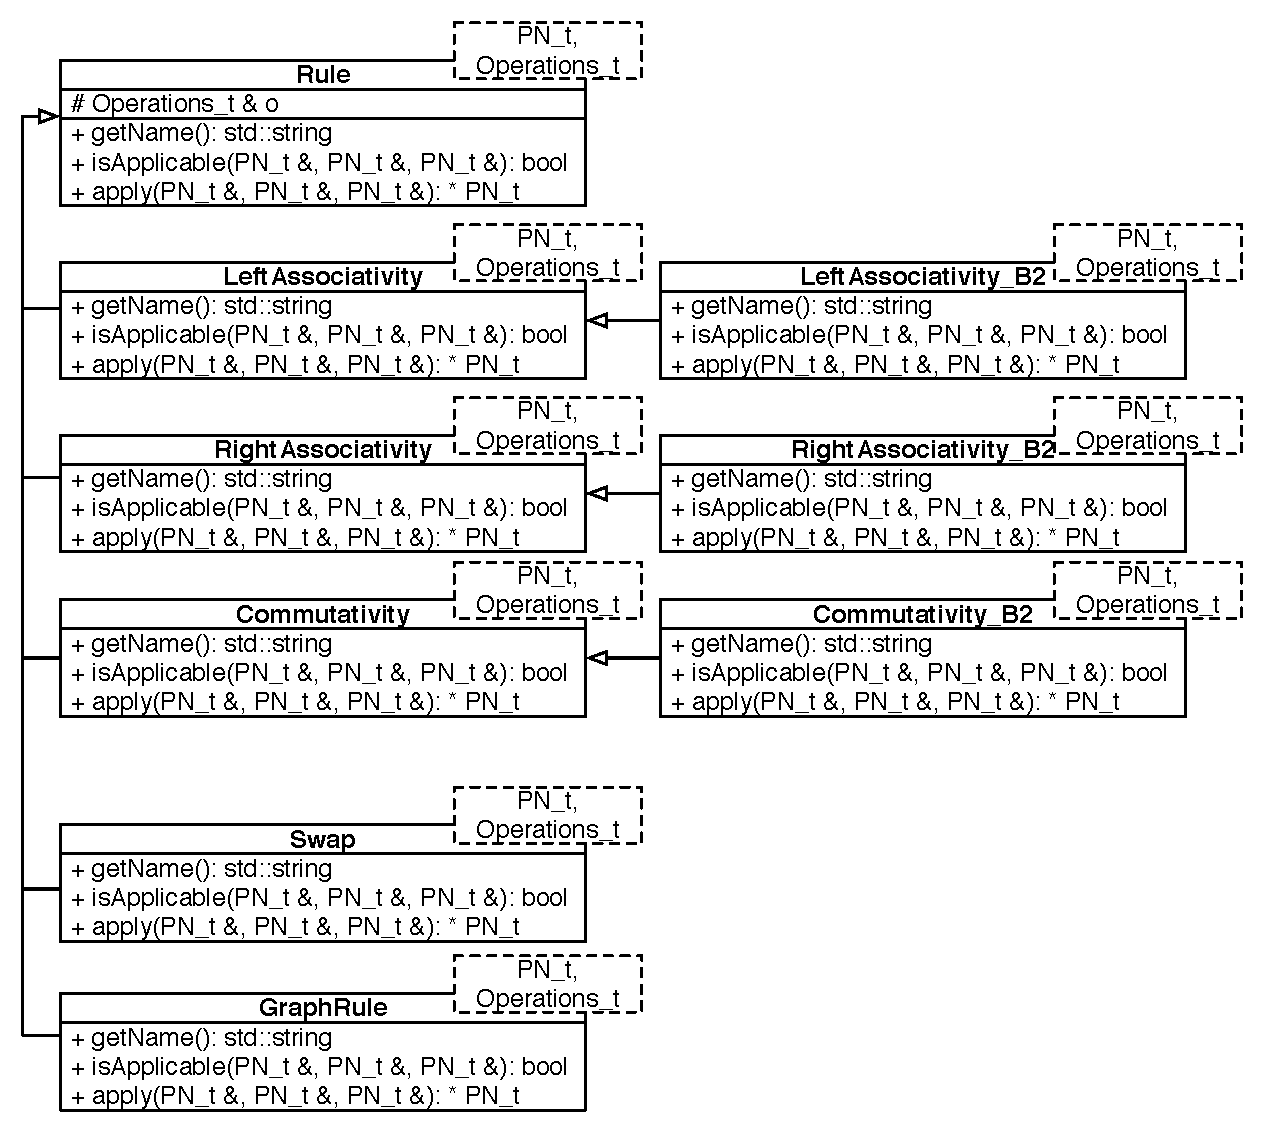
\includegraphics[scale=0.75]{04_Implementierung/00_media/Rules.pdf}
  \caption{Klassendiagramm: Regeln}
  \label{RuleClassDiagram}
\end{figure}

Die einzelnen Regeln, die Teil der Regelmengen sind, werden jeweils in einer eignen Klasse abgelegt. Aktuell sind acht Regeln vorhanden: (1) \texttt{Commutativity}, (2) \texttt{Left Associativity}, (3) \texttt{Right\-Associativity}, (4) \texttt{Commu\-tativity B2}, (5) \texttt{Left\-Associtativity-B2}, (6) \texttt{Right\-Associativity-B2}, (7) \texttt{Exchange}, (8) \texttt{Graph Rule}. Die Zuordnung der Regeln zu den unterschiedlichen Regelmenegen wurde in \ref{sec:RuleImplementation} erklärt und in Abb. \ref{RuleSetClass} veranschaulicht.

Einer der konzeptionellen Unterschiede zwischen den in Kapietl 3 beschriebenen Regeln und den hier implementierten Regeln ist, dass die hier implementierten Regeln per se kreuzproduktfrei sind. Es wird bereits vor der Anwendung einer Regel geprüft, ob eine Regel ein Kreuzprodukt generieren wird, nur wenn das Ergebnis kreuzproduktfrei sein wird, kommt die Regel zur Anwendung. Dieses Vorgehen ermöglicht,  bereits frühzeitig die Generierung von Plänen abzubrechen, wenn die erzeugten Pläne nicht zielführend sind. Da die Regeln nicht prüfen, ob nach ihrer Anwendung ein Kreuzprodukt entstanden ist, sondern diese Prüfung bereits zuvor geschieht, werden die Regelmengen im Folgenden auch nicht mit dem Post-Fix -CPS bezeichnet.

\subsubsection{Implementierung}


\begin{figure}[ht]
  \centering
  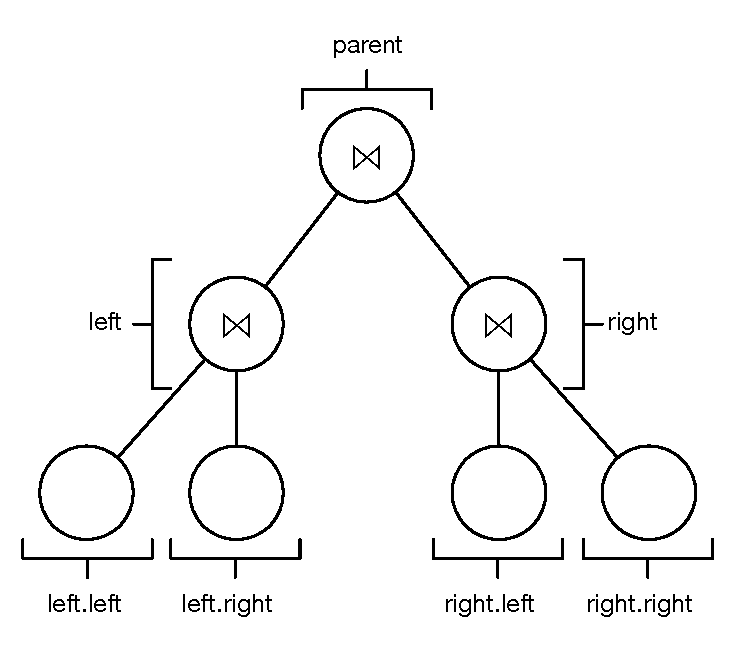
\includegraphics[scale=0.75]{04_Implementierung/00_media/Plan.pdf}
  \caption{Plandiagramm: Einfacher Beispiel-Plan}
  \label{SimplePlan}
\end{figure}


Auch bei den Regeln erben alle Regeln direkt oder - und das ist neu - indirekt von der Klasse \texttt{Rule}. Die Organisation der Klassen ist in Abb. \ref{RuleClassDiagram} dargestellt. Alle Regeln implementieren das Interface, das durch die abstrakte Klasse \texttt{Rule} vorgegeben ist. Durch die Methode \texttt{getName()} wird der Name der jeweiligen Regel zurückgeliefert. Wie bei anderen Implementierungen sind die Regeln in zwei Teilen organisiert. Mit Hilfe der Methode \texttt{isApplicable} kann festgestellt werden, ob eine Regel anwendbar ist, Die Methode \texttt{apply} wendet die Regel an und liefert einen Planknoten zurück. Kreuzprodukte werden nicht wie bei \cite{shanbhag2014optimizing} erst nach der Bildung neuer Pläne geprüft, sondern schon im \texttt{isApplicable}-Teil. So werden ausschließlich kreuzproduktfreie Bäume gebildet. Der Planknoten selbst, sowie die Operationen, die zur Erzeugung eines neuen Plans führen, können durch Template Parameter ausgetauscht werden. So ist es möglich andere Planknoten zu verwenden und die Funktionsweise von Operationen wie \texttt{JOIN} völlig neu zu bestimmen.


Die konkrete Implementierung der Regeln lässt sich am besten am Beispiel eines konkreten Plans erläutern. Ein solch konkreter Plan ist in Abb. \ref{SimplePlan} zu sehen. Der oberste Knoten wird als \textit{parent} bezeichnet. Ihm sind zwei Äquivalenzklassen untergeordnet \textit{parent.left} und \textit{parent.right}. 

Wie bereits bekannt, kann eine Äquivalenzklasse mehrere Planknoten beheimaten. Bei der Ausführung der Regeln wird ein Planknoten nach dem anderen betrachtet und für diesen eine Regel ausgeführt. In diesem Falle ist der Äquivalenzklasse \textit{parent.left} und \textit{parent.right} je nur ein Planknoten zugeordnet. Diesen Planknoten sind selbst wieder je zwei Äquivalenzklassen untergeordnet.


Bei der Ausführung einer Regeln wird in die konkrete Regel der \textit{parent} und je ein konkreter Planknoten der untergeordneten Äuqivalenzklassen übergeben. Im konkreten Fall sind das \textit{left} und \textit{right}





\subsubsection{Implementierung von Kommutativität}

Bei der Regel Kommutativität wird nur auf den \textit{Parent} und dessen Äquivalenzklassen geachtet. Im \texttt{isApplicable}-Teil der Regel wird zuerst geprüft, ob die Operation des \textit{parent}-Knoten ein JOIN ist. Wenn das der Fall ist, wird noch geprüft, ob die linke und rechte Äquivalenzklasse überlappen. Dies geschieht mit der Methode \texttt{isOverlapping}. Liefert auch diese Methode \texttt{true} zurück, kann die Regel angewendet werden.

Bei der Regelanwendung kommt wie bei anderen Regeln die Hilfs Klasse \texttt{Operations} vor. Mit ihrer Hilfe wird ein neuer Planknoten erzeugt, der die linke und rechte Äquivalenzklasse des Planknoten vertauscht.

Die genaue Implementierung der Regel ist in \ref{CommutativityCode} zu sehen.


\begin{figure}[ht]
\lstinputlisting{04_Implementierung/00_media/Commutativity.h}
\caption{C++: Kommutativität}
\label{CommutativityCode}
\end{figure}




\subsubsection{Implementierung von Assoziativität}

Bei der linken Assoziativität wird zuerst geprüft, ob der Operator des \textit{parent}-Knotens ein JOIN ist. Wenn dies der Fall und der \textit{left}-Knoten ein JOIN Operator ist, dann wird geprüft, ob die rechte Äquivalenzklasse des \textit{parent}-Knoten mit der rechten Äquivalenzklasse des \textit{left}-Knotens überlappt. Falls alles zutrifft ist die Regel anwendbar.

Bei der Anwendung wird zuerst ein neuer Planknoten erzeugt, der direkt einer neuen Äquivalenzklasse zugeordnet wird. Der neue Planknoten repräsentiert den Join zwischen der rechten Äquivalenzklasse des \textit{left}-Knotens und der rechten Äquivalenzklasse des \textit{parent}-Knotens. Die neugebildete Klasse wird zum rechten Teil eines wiederum neuen Äquivalenzknotens, der den linken \textit{parent}-Teil mit der neuen Äquivalenzklasse joint. Das Ergebnis ist linke Kommutatvitität.

Diese Implementierung ist auch in \ref{LeftAssociativityCode} nachzuvollziehen und funktioniert analog zur Implementierung der rechten Assoziativität, die in \ref{RightAssociativityCode} zu sehen ist.


\begin{figure}[ht]
\lstinputlisting{04_Implementierung/00_media/LeftAssociativity.h}
\caption{C++: Linke Assoziativität}
\label{LeftAssociativityCode}
\end{figure}

\begin{figure}[ht]
\lstinputlisting{04_Implementierung/00_media/RightAssociativity.h}
\caption{C++: Rechte Assoziativität}
\label{RightAssociativityCode}
\end{figure}




\subsubsection{Implementierung von abgeleiteten RS-B2 Regeln}

Die Regeln von RS-B2 unterscheiden sich maßgeblich dadurch, dass nach Anwendung einer Regel andere Regeln von der Anwendung auf den neuen Knoten ausgeschlossen sind. Wie bereits beschrieben, ist die Information, ob eine Regel auf einen Planknoten bereits angewendet wurde im Planknoten selbst gespeichert. Die dafür vorgesehenen boolean Variablen, können mit Hilfe der Methoden \texttt{disable\-All\-Rules()} und \texttt{disable\-All\-And\-Enable\-Commutativity()} auf \texttt{false} gesetzt werden. Mit den Methoden \texttt{is[RULENAME]Enabled()} lässt sich für jede Regel prüfen, ob diese auch benutzt werden darf.

Die konkrete Implementierung sieht vor, dass die Regeln \texttt{Commutativity\-B2, Left\-Associativity\-B2} und \texttt{Right\-Associativity} direkt von \texttt{Commutativity}, \texttt{}{Left\-Associativity} und \texttt{Right\-Associativity} erben. Bei dem Aufruf von \texttt{is\-Applicable} wird zuerst geprüft, ob die Regel \texttt{enabled} ist mit Hilfe der dafür vorgesehenen Zugriffsmethode. Wenn das der Fall ist, kann die geerbte Methode aufgerufen werden und so geprüft werden, ob auch alle anderen Voraussetzungen erfüllt sind.

Bei der Ausführung der \texttt{apply}-Methode wird  zuerst die geerbte Methode ausgeführt und dann auf diese Methode die Notwendige disable Methode aufgerufen, um für diesen Knoten die Regel zu deaktivieren.

Konkret kann diese Implementierung in \ref{CommutativityB2Code} nachvollzogen werden.


\begin{figure}[ht]
\lstinputlisting{04_Implementierung/00_media/Commutativity_B2.h}
\caption{C++: Kommutativität B2}
\label{CommutativityB2Code}
\end{figure}



\subsubsection{Implementierung der Exchange Rule}
Die Exchange Regel hingegen erbt nicht von anderen Regeln, sondern ist neu implementiert worden. Auch diese Implementierung sieht wieder vor, dass im \texttt{is\-Applicable}-Teil geprüft wird, ob sowohl der \textit{parent}, \textit{left} als auch der \textit{right} Knoten als Operatoren Joins verwenden. Ist dies der Fall und überlappt die rechten Äquivalenzklassen des \textit{left} und \textit{right}-Knoten, dann kann die Regel ausgeführt werden. Vorausgesetzt eine vorhergehende Prüfung mit der Methode \texttt{is\-Exchange\-Applicable()} war erfolgreich. 




\subsection{GraphRule / RS-Graph}

\begin{figure}[ht]
\lstinputlisting{04_Implementierung/00_media/GraphRuleApply.h}
\caption{C++: GraphRule apply}
\label{GraphRuleApply}
\end{figure}

Wie auch in Kapitel 3 beschrieben, wurde eine weitere Regel implementiert GraphRule. Für diese Regel wurde eine eigene Regelmenge gebildet. Diese Regelmenge erfüllt das vorgegebene Interface und kann so genutzt werden, wie andere Regelmengen. Diese Erweiterung zeigt per se die Erweiterbarkeit des Prototpyen.

Die Implementierung der GraphRule geschah in zwei Schritten: Ähnlich wie bei der in Kapitel 3 implementierten GraphRule wurde hier das Interface erfüllt, das es ermöglicht einen Top-Down-Enumerator als Transformationsregel auszuführen.




Wie in Abbildung \ref{GraphRuleApply} zu erkennen, wird sowohl das Interface \texttt{Rule} eingehalten, als auch die Implementierung aus Kapitel 3 übernommen. Wie zu erwarten, ist die Methode \texttt{partition} ähnlich schlank wie in ihrer Vorlage implementiert. In Zeile 3 wird die Methode MinCutConservative aufgerufen, die für die tatsächliche Ausführung der Partitionierung verantwortlich ist.



\begin{figure}[ht]
\lstinputlisting{04_Implementierung/00_media/MinCutConservative.h}
\caption{C++: MinCutConservative / Partitionierung}
\label{fig:MinCutConservative}
\end{figure}

Bei dem Zusammenbau der Bäume mit Hilfe der Methode \texttt{createTree} werden die einzelnen Bäume aus Äquivalenzklassen und Planknoten zustammgesetzt. Auf oberster Ebene wird eine Äquivalenzklasse gebildet, die jedoch, um das Interface zu erfüllen nicht zurückgeben wird. Stattdessen wird der erste Planknoten übergeben, der mit Hilfe des Zeigers \texttt{\_next} auf den nächsten Knoten zeigt und somit den ganzen Baum übergeben kann.